\documentclass[10pt]{article}
\usepackage{fancyhdr}
\usepackage{amsmath}
\usepackage{graphicx}
\pagestyle{fancy}
\headheight 35pt
\parskip 10pt \parindent 0pt 
\lhead{Classical Mechanics HW 4}
\chead{Andrei Ilyashenko}
\rhead{10-10-2010}
\cfoot{\thepage}

\begin{document}
\textbf{Chap 8 der 3}\\
If we wish to use $\dot p_i$ and $\dot q_i$ as our independent variables, then
We will need the following Hamiltonian.
\begin{align*}
  G(\dot p_i, \dot q_i, t) &= q_i\dot p_i -L.\\
\end{align*}
Its differential is
\begin{align*}
  dG &= \dot p_i dq_i + q_id\dot p_i -\dot p_idq_i-p_id\dot q_i-\frac{\partial L}{\partial t}dt\\
  dG &=  q_id\dot p_i -p_id\dot q_i-\frac{\partial L}{\partial t}dt.
\end{align*}
Of course we can also find the differential of G by taking partial derivatives 
with respect to $\dot p_i$ and $\dot q_i$.  So, we have the following equations
\begin{align*}
  q_i &= \frac{\partial G}{\partial\dot p_i}\\
  -p_i &= \frac{\partial G}{\partial\dot q_i}\\
  -\frac{\partial L}{\partial t} &= \frac{\partial H}{\partial t}.
\end{align*}
\textbf{Chap 8 Ex 19}\\
\begin{figure}[h!]
    \centering
    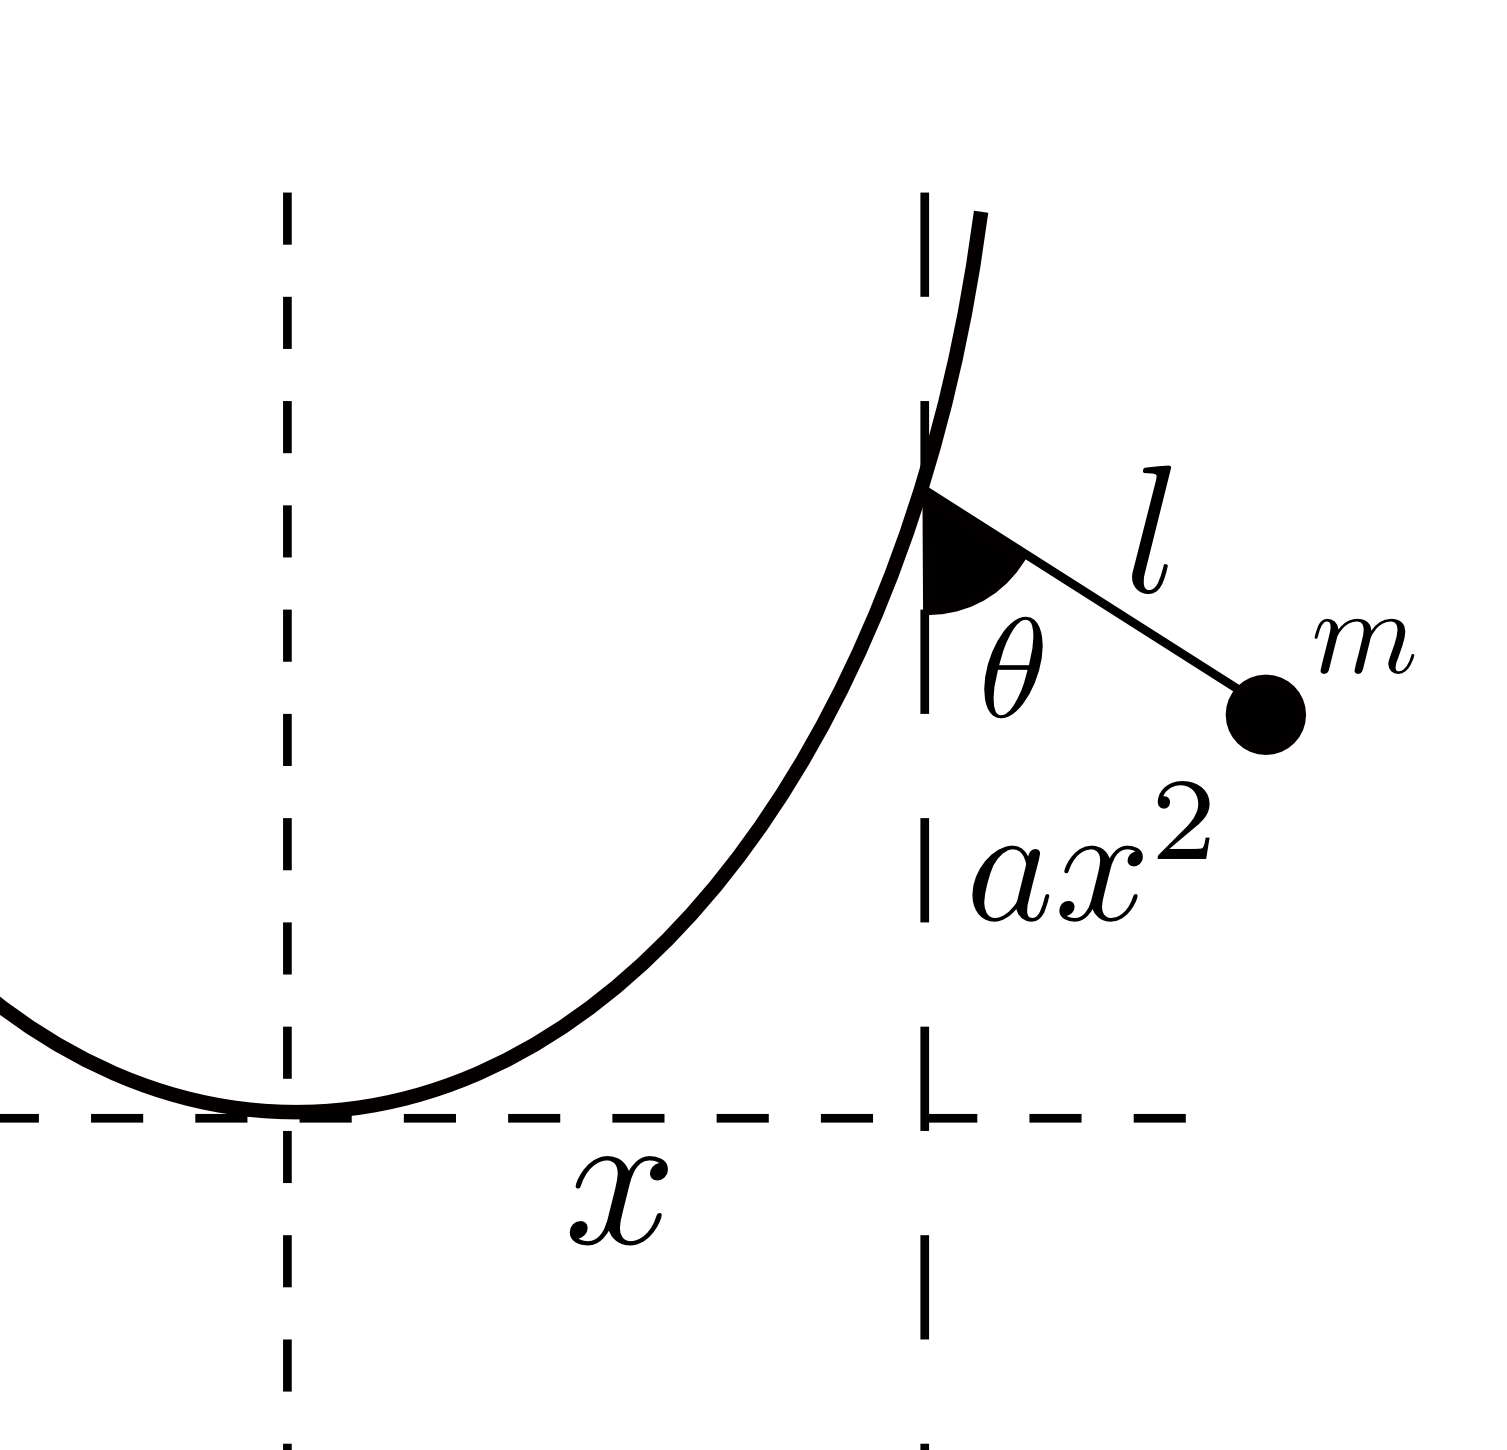
\includegraphics[width=0.7\textwidth]{8-19.png}
    \caption{This figure shows the generalized coordinates for the pendulum problem.}
  \label{fig:8-19}
\end{figure}
So, the location of the mass is given by $\theta$ and $x$, see fig. \ref{fig:8-19} for a picture.
\begin{align*}
  x_{\rm{particle}} &= x+l\cos\theta\\
  z &= ax^2-l\cos\theta.
\end{align*}
So, the potential and kinetic energies are
\begin{align*}
  T &= \frac{1}{2}m(\dot x_{\rm{particle}}^2 + \dot z^2)\\
    &= \frac{1}{2}m\left( \left(\dot x-l\dot\theta\sin\theta  \right)^2 + \left(2ax\dot x+l\dot\theta\sin\theta  \right)^2  \right)\\
    \\
  V &= mgz\\
    &= mg\left( ax^2-l\cos\theta \right).
\end{align*}
So, the canonical momenta are
\begin{align*}
  p_{x} &= 
    m\left( \left(\dot x-l\dot\theta\sin\theta  \right) + 2ax\left(2ax\dot x+l\dot\theta\sin\theta  \right)  \right)\\
    \\
  p_{\theta} &= 
    ml\sin\theta\left( -\left(\dot x-l\dot\theta\sin\theta  \right) + \left(2ax\dot x+l\dot\theta\sin\theta  \right)  \right)\\
    \\
\end{align*}
Thus, the Hamiltonian is
\begin{align*}
  H &= \dot x p_x + \dot\theta p_{\theta} - L\\
    &= \dot x p_x + \dot\theta p_{\theta} - T + V\\
    &= \dot x p_x + \dot\theta p_{\theta} - \frac{1}{2}\left( \dot x p_x + \dot\theta d\theta \right) + mg\left( ax^2-l\cos\theta \right)\\
    &= \frac{1}{2}\left( \dot x p_x + \dot\theta d\theta \right) + mg\left( ax^2-l\cos\theta \right)\\
    &= \frac{1}{2ml^2\sin^2\theta(1+2ax)^2}\left( \left(p_{\theta}+lp_x\sin\theta  \right)^2 + \left(2axp_{\theta}-lp_x\sin\theta  \right)^2  \right) + mg\left( ax^2-l\cos\theta \right)\\
    &= \frac{\mathcal{A}}{2}\left( \left(p_{\theta}+lp_x\sin\theta  \right)^2 + \left(2axp_{\theta}-lp_x\sin\theta  \right)^2  \right) + mg\left( ax^2-l\cos\theta \right).
\end{align*}
So, essentially we replaced $\dot\theta$ with $p_x$ and $\dot x$ with $p_{\theta}$, and had to change the sign of the $p_x$ terms.
Also notice that as expected the Hamiltonian was just the total energy. The Hamiltonian equations of motion are
\begin{align*}
  \dot x &= \mathcal{A}l\sin\theta\left(\left(p_{\theta}+lp_x\sin\theta  \right) - \left(2axp_{\theta}-lp_x\sin\theta  \right)  \right)\\
  \dot \theta &= \mathcal{A}\left(\left(p_{\theta}+lp_x\sin\theta  \right) + 2ax \left(2axp_{\theta}-lp_x\sin\theta  \right)  \right)\\
  -\dot p_x &= \mathcal{A}\left( 2ap_{\theta}\left(2axp_{\theta}+lp_x\sin\theta  \right)  \right) + 2axmg\\
  -\dot p_{\theta} &= \mathcal{A}lp_x\cos\theta\left( \left(p_{\theta}+lp_x\sin\theta  \right) - \left(2axp_{\theta}-lp_x\sin\theta  \right)  \right)+ mg\left( ax^2-l\cos\theta \right)
\end{align*}
A quick check of the units shows that $a$ must have units of inverse length, but that otherwise the units match.
\textbf{Chap 8 Ex 23}\\
\textbf{a)}\\
Notice that the curl of $A$ as defined in the book will give a uniform magnetic field of strength $B$
pointing in the z direction.  Also, $A$ can be defined as $A=(B\times(a_1 x \hat i + a_2 y \hat j))$, with
the condition that $a_1+a_2=1$, so the book chose $a_1=a_2=\frac{1}{2}$, but one could also choose
$a_1=0$ and $a_2=1$ and that could simplify the problem.\\
\\
The kinetic and potential energies are
\begin{align*}
  T &= \frac{1}{2}m(\dot x^2+ \dot y^2)\\
  V &= V(r) - q A\dot v\\
  &= V(r) - \frac{q B}{2} (x\dot y-\dot xy).
\end{align*}
So, the canonical momentum are
\begin{align*}
  p_x &= m\dot x - \frac{q B}{2} y\\
  p_y &= m\dot y + \frac{q B}{2} x.
\end{align*}
So, $\dot x$, and $\dot y$ are
\begin{align*}
  m\dot x &= p_x + \frac{q B}{2} y\\
  m\dot y &= p_y - \frac{q B}{2} x.
\end{align*}
Hamiltonian should be equal to the total energy again, but lets use the general formula
one more time.  
\begin{align*}
  H &= p_iq_i-L\\
  H &= \frac{1}{2m}\left[ p_x^2+p_y^2-qB(yp_x-xp_y)-\frac{q^2B^2}{4}(x^2+y^2) \right].
\end{align*}
All of the algebra has been omitted because it was done on a computer, and again as
expected the Hamiltonian is the total energy.\\
\textbf{b)}\\
We can derived $\omega$, where $\omega$ is the angular velocity of the rotating body frame.  We know
that there must be a centripetal force in order for the particle to move in a circle, the magnetic field 
provides this force, but it can also be written in terms of $\omega$.  Thus, we have
\begin{align*}
  F_c &= -m\frac{d}{dt}(\omega r)\\
  e\dot rB &= -m\frac{d}{dt}(\omega r)\\
  erB &= -m(\omega r)\\
  \omega &= -\frac{eB}{m}.
\end{align*}
Assuming that $m$, $e$, and $B$ are fixed.  This is where the book gets the $\omega$ value.  So, it turns
out that the magnetic force the charged particle experiences will cause it to rotate with angular velocity 
$-\frac{eB}{m}$ that is independent of its position or velocity, which means if we use the non-inertial
reference frame the book suggests, the fictitious centrifugal forces should cancel with the magnetic force.  
We will define one general coordinate: $r$.  Notice that there are three forces besides the central potential
acting on the particle.  They are the centrifugal force, the Coriolis force, and the magnetic force.  Their magnitudes are
\begin{align*}
  F_{\rm{magnetic}} &= 2eB\dot r\hat\theta- eBr\omega\hat r\\
  F_{\rm{centrefugal}} &= m\omega^2 r\hat r\\
  F_{\rm{coriolis}} &= -2m\omega\dot r\hat\theta.
\end{align*}
Notice that all these forces perfectly cancel each other. So, our kinetic and potential energies are given by
\begin{align*}
  T &= \frac{1}{2}m(\dot r^2+r^2\omega^2)\\
  V &= V(r).
\end{align*}
\textbf{Chap 8 Ex 24}\\
This problem involves a two dimensional motion because the mass can move along the track, and
the cylinder can spin.  Let generalized coordinates be $l$, the distance the mass has moved along
the track, and $\theta$ the angle that the cylinder has rotated through.  The kinetic and potential
energies are given by
\begin{align*}
  T &= \frac{1}{2} \left( M\frac{a^2}{2}\omega^2+mf'(l)^2\dot l^2+m(g'(l)\dot l+\omega a)^2 \right)\\
    &= \frac{1}{2} \left( M\frac{a^2}{2}\omega^2+mf'(l)^2\dot l^2+gm'(l)\dot l^2 + 2mg'(l)\omega a\dot l + m\omega^2 a^2 \right)\\
    &= \frac{1}{2} \left( M\frac{a^2}{2}\omega^2+m\dot l^2 + 2mg'(l)\omega a\dot l + m\omega^2 a^2 \right)\\
  V &= -mgf(l),
\end{align*}
where $M$ is the mass of the cylinder, and $f$ is a monotonically increasing function that computes the vertical
distance the mass has travelled given the distance it has moved along the track, and $g$ is a function that 
computes the angular distance the mass has rotated.  These functions depends on the shape of the track.  So, 
the canonical momenta are
\begin{align*}
  p_l &= m\dot l + g'(l)m\omega a\\
  p_{\theta} &= \left( M\frac{a^2}{2}\omega+ma^2\omega+mg'(l)\dot la \right)\\
\end{align*}
The Hamiltonian will be the total energy since the Lagrangian does not depend on time, and all forces are derivable
from a conservative potential.  Also keep in mind that since $f$ and $g$ return a distance, their derivative with
respect to $l$ will be unitless.
\begin{align*}
  H &= T+V\\
    &= \frac{1}{2} \left( M\frac{a^2}{2}\omega^2+m\dot l^2 + 2mg'(l)\omega a\dot l + m\omega^2 a^2 \right)-mgf(l)\\
    &= \frac{-1}{a^2 m ((-1 + g^2) m - M) } \left( M\frac{a^2}{2}p_l^2+mp_{\theta}^2 - 2mg'(l)p_l ap_{\theta} +m p_l^2 a^2 \right)-mgf(l)\\
    &= \mathcal{A} \left( M\frac{a^2}{2}p_l^2+mp_{\theta}^2 - 2mg'(l)p_l ap_{\theta} +m p_l^2 a^2 \right)-mgf(l)\\
\end{align*}
So, the Hamiltonian equations of motion are
\begin{align*}
  \dot l &= \mathcal{A} \left( Ma^2p_l - 2mg'(l) ap_{\theta} +2m p_l a^2 \right)\\
  \dot \theta &= \mathcal{A} \left( 2mp_{\theta} - 2mg'(l)p_l a \right)\\
  -\dot p_l &= -mgf'(l) - \mathcal{A}2mg''(l)p_l ap_{\theta}\\
  -\dot p_{\theta} &= 0.
\end{align*}
I cannot find a solution without knowing $g$ and $f$.  Lets assume that $f'(l)=c$ and $g'(l)=b$, so 
$g''(l)=0$ and $c^2+b^2=1$.  This means that the track is shaped in such a way that the ratio of
tangential to vertical motion remains constant.  If this is the case, our equations of motion become.
\begin{align*}
  \dot l &= \mathcal{A} \left( Ma^2p_l - 2mb ap_{\theta} +2m p_l a^2 \right)\\
  \dot \theta &= \mathcal{A} \left( 2mp_{\theta} - 2mbp_l a \right)\\
  -\dot p_l &= -mgc\\
  -\dot p_{\theta} &= 0.
\end{align*}
So, the canonical momentum is given by
\begin{align*}
  p_{\theta} &= \rm{Constant}\\
  p_l &= mgct.
\end{align*}
From here, the canonical momentum can by substituted into the equations for $\dot l$ and $\dot\theta$,
and then we will have $\dot l$ and $\dot\theta$ as function of time.  If we integrate once, we will
even have $l$ and $\theta$ as functions of time, but this algebra is unnecessary if you want a 
qualitative understanding of the motion.  Basically, as time goes on, the mass picks up speed along
the track, and the cylinder-mass system starts spinning in the counter clockwise direction the rate
at which the system gains angular momentum depends on $cb$, and if $cb=0$ (as in a flat track or a 
track going straight down), then there is no change in angular momentum.
\textbf{Chap 8 Ex 26}\\
\textbf{a)}\\
Lets take the generalized coordinate to be $x$, the distance the mass is from the center of the system
with values of $x$ to the right of the center being positive.  The kinetic and potential energies are
\begin{align*}
  T &= \frac{1}{2}m\dot x^2\\
  U &= \frac{1}{2}k_1\left( x-\frac{a}{2} \right)^2 + \frac{1}{2}k_2\left( x+\frac{a}{2} \right)^2
\end{align*}
The Lagrangian is
\begin{align*}
  L &= T - U\\
  &= \frac{1}{2}m\dot x^2 - \frac{1}{2}k_1\left( x-\frac{a}{2} \right)^2 - \frac{1}{2}k_2\left( x+\frac{a}{2} \right)^2.
\end{align*}
The canonical momentum is $p_x = m\dot x$, and the Hamiltonian is
\begin{align*}
  H &= T + U\\
  &= \frac{p_x^2}{2m} + \frac{1}{2}k_1\left( x-\frac{a}{2} \right)^2 + \frac{1}{2}k_2\left( x+\frac{a}{2} \right)^2.
\end{align*}
The energy is conserved, since the Hamiltonian is just the total energy, and does not depend on time.\\
\textbf{b)}\\
Assuming that this coordinate is 0 at the center of the system, the kinetic and potential energies are
\begin{align*}
  T &= \frac{1}{2}m\left( \dot Q \right)^2\\
  T &= \frac{1}{2}m\left( \dot q - \omega b\cos\omega t \right)^2\\
  U &= \frac{1}{2}k_1\left( Q-\frac{a}{2} \right)^2 + \frac{1}{2}k_2\left( Q+\frac{a}{2} \right)^2
\end{align*}
The Lagrangian is
\begin{align*}
  L &= T-U\\
   &= \frac{1}{2}m\left( \dot Q \right)^2 - \frac{1}{2}k_1\left( Q-\frac{a}{2} \right)^2 - \frac{1}{2}k_2\left( Q+\frac{a}{2} \right)^2.
\end{align*}
The canonical momentum is $p_Q = m\dot Q$.  The Hamiltonian is
\begin{align*}
  H &= \dot Q p_Q - L\\
   &= \dot Q p_Q - \frac{1}{2}m\left( \dot Q \right)^2 + \frac{1}{2}k_1\left( Q-\frac{a}{2} \right)^2 + \frac{1}{2}k_2\left( Q+\frac{a}{2} \right)^2\\
   &= \frac{1}{2}m\left( \dot Q \right)^2 + \frac{1}{2}k_1\left( Q-\frac{a}{2} \right)^2 + \frac{1}{2}k_2\left( Q+\frac{a}{2} \right)^2.
\end{align*}
The Hamiltonian is not conserved, since it is an explicit function of time, the energy will also not be conserved.

\end{document}
